\chapter{Metodología de Desarrollo}
\label{chap:metodologia}
%\endinput
 
Para el desarrollo de este trabajo se opt\'o por un modelo de desarrollo de tipo incremental (que resulta iterativo por naturaleza).
En cada iteraci\'on, se optimiz\'o el dise\~no y se fueron agregando nuevas funcionalidades y capacidades al sistema.\\

El problema que se propone resolver, requiere de la implementaci\'on de distintos algoritmos en una estructura en donde los resultados de un m\'odulo se utilizan en el siguiente. Esto implica que para un an\'alisis completo cada una de las instancias debi\'o estar previamente validada. \\

No obstante, las salidas de los m\'odulos que eran ingesta de otros m\'odulos pod\'ian reemplazarse por datos ya conocidos, y as\'i desarrollar y validar el m\'odulo siguiente, mientras se analizaba en paralelo c\'omo mejorar o corregir los resultados no satisfactorios. De esta manera se fue armando el cuerpo general del software a gran escala, y luego se fue revisando y afinando cada uno de los paquetes.\\

Esta forma de trabajo permiti\'o dividir la complejidad del proyecto, y a su vez, desarrollar un conjunto de bibliotecas f\'acilmente modificables, sin alterar la estructura central.



\section{Plan de Desarrollo}

Dado que el trabajo se realizaba en el contexto de la maestr\'ia en general y que las tareas y los cronogramas se modificaban frecuentemente, ajust\'andose al dictado de cursos y tareas de un proyecto integrador que tambi\'en formaba parte del ciclo lectivo; en un principio no era posible armar un cronograma fijo de las tareas.\\

Se planific\'o una distribuci\'on horaria (Fig. \ref{fig:disths}) y una planificaci\'on general (Fig. \ref{fig:plan2016}) para los semestres I, III y IV del año 2016.

\begin{figure}[!h]
  \centering
  \fbox{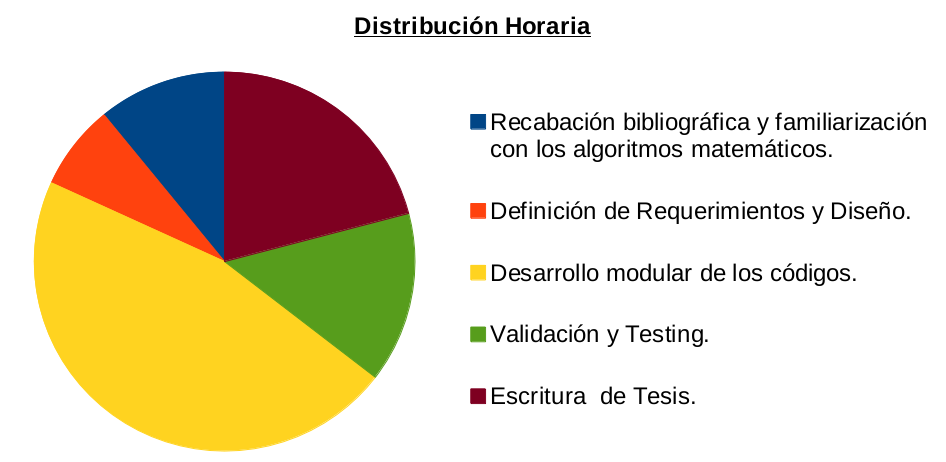
\includegraphics[width=0.8\textwidth]{imagenes/distribucionhs}}
  \caption{Planificaci\'on de la distribuci\'on del total de horas asignadas dentro de la maestr\'ia al desarrollo y la escritura del trabajo de tesis.}
  \label{fig:disths}
\end{figure}

\begin{figure}[H]
  \centering
  \fbox{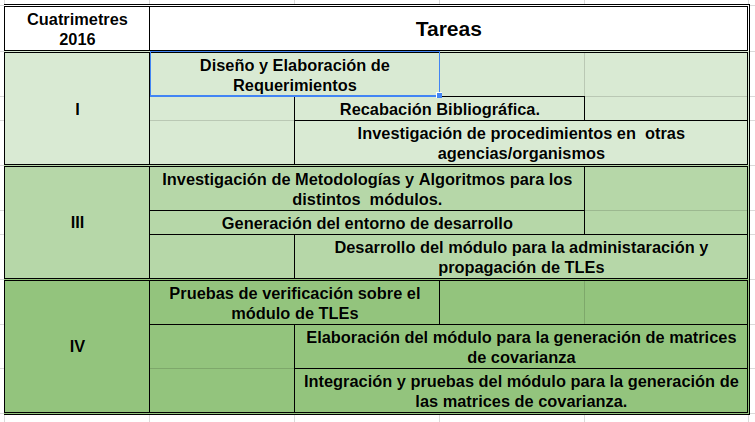
\includegraphics[width=\textwidth]{imagenes/plan2016}}
  \caption{Planificaci\'on de las tareas agrupadas por semestres para el año 2016}
  \label{fig:plan2016}
\end{figure}

Ya a comienzos del año 2017 se contaba con un cronograma fijo que pautaba tres semanas por mes de dedicaci\'on exclusiva a la elaboraci\'on de la tesis. Eso permiti\'o realizar una planificaci\'on semanal (Fig. \ref{fig:plan2017}) de las tareas. 

\begin{figure}[H]
  \centering
  \fbox{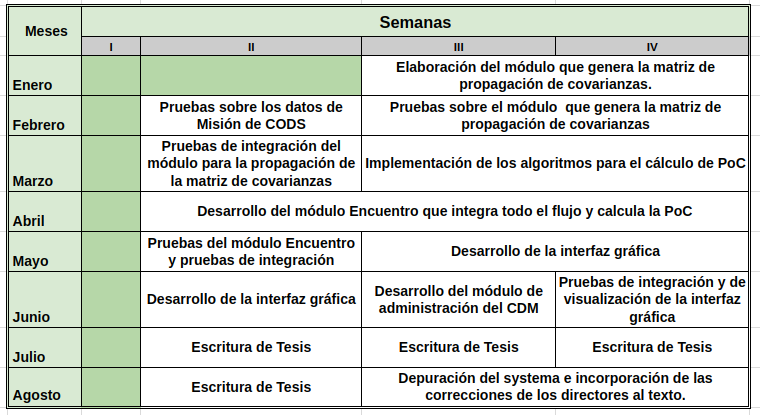
\includegraphics[width=\textwidth]{imagenes/plan2017}}
  \caption{Planificaci\'on de las tareas agrupadas por semanas para el año 2017}
  \label{fig:plan2017}
\end{figure}

\section{Entorno de Desarrollo}\label{sec:entorno}

Para el desarrollo se utiliz\'o:\\
\begin{itemize}
 \item Plataforma de Desarrollo (\ac{IDE}): Eclipse Ver. 3.8.1.
 \item Lenguaje de Programaci\'on: Python 2.7
 \item Biblioteca de Interfaz gr\'afica: QT por medio del enlace PyQT.
 \item Gestor de Configuraci\'on: Git.
\end{itemize}

\subsection*{Eclipse}
Eclipse (Ver. 3.8.1) es una plataforma de desarrollo multiplataforma ampliamente utilizada y ya muy madura, cuya estructura de perspectivas, editores y vistas, facilita el desarrollo en distintos lenguajes de programaci\'on. En este trabajo se incorpor\'o el IDE para python, {\it{Pydev}}.\\

Eclipse ofrece excelentes capacidades para la gesti\'on de proyectos, permitiendo incorporar en un mismo proyecto distintos archivos y documentaci\'on, que, en esta tesis, agrup\'o no s\'olo los datos de entrada y salida, como los TLE, los CDM o los productos orbitales; sino que tambi\'en incluy\'o todos los ploteos y gr\'aficos que resultaban de los procesamientos y la propia documentaci\'on referida a la escritura de este documento. Esto fue muy productivo en lo que respecta al control de versiones, ya que se aprovech\'o el hecho de que Eclipse ya tiene incorporado el gestor Git.
Cabe destacar también, que cuenta con una excelente herramientas de depuraci\'on.\\

\subsection*{Python}
El lenguaje de programaci\'on Python se destaca en sus capacidades tanto de c\'alculo como de manejo de texto. Esto agiliza mucho los procesos que involucran el manejo de tablas de datos plasmadas en texto plano, como son por ejemplo los datos TLE y las efem\'erides orbitales que se generan como productos del departamento de Din\'amica Orbital. As\'i mismo facilita el manejo de las nomenclaturas de los distintos archivos de datos o im\'agenes generadas.\\

Existen numerosas, potentes y optimizadas bibliotecas para la realizaci\'on de c\'alculos, y el tratamiento vectorial. En nuestro caso se aprovech\'o particularmente la biblioteca {\it{numpy}}, y muy poco de {\it{scipy}} espec\'ificamente, para interpolar datos.
Finalmente su utilizaci\'on masiva permite tener acceso r\'apido a sus potencialidades.\\

\subsection*{QT}
Para el desarrollo de la interfaz gr\'afica se utiliz\'o QT, a trav\'es del enlace PyQT.\\
QT es un framework ampliamente utilizado para el desarrollo de aplicaciones multiplataforma. Cuenta con mucha contribuci\'on de la comunidad y est\'a soportado por Nokia.\\

Su mecanismo de conexión de señales y eventos es simple, esto permite definir los eventos sencillos en la estructura del GUI, y luego invocar el c\'odigo python con las acciones m\'as avanzadas. Subyace su implementaci\'on en C++ que muchas veces dificulta la comprensi\'on para los que estamos familiarizados con la l\'ogica del python, y lo mismo ocurre con la documentaci\'on y prevalecen los ejemplos para C++.\\

\subsection*{Git}
Si bien, esta herramienta no fue aprovechada en todo su potencial en este trabajo, por tratarse de un proyecto sencillo y desarrollada por dos personas, fue fundamental para agilizar la posibilidad de trabajar desde cualquier computadora, siempre en la \'ultima versi\'on del proyecto.
As\'i mismo, el trabajo con control de versiones, permiti\'o realizar distintas pruebas e implementaciones que luego se descartaron o se quitaron del producto final, pero que pueden ser reutilizados en futuros proyectos. En particular, en la utilizaci\'on de la interfaz intermedia que fue generada para una \'agil evaluaci\'on de los resultados parciales.\\





% \section{Iteraci\'on}
% Ya conocido el planteo del problema, las distintas maneras de abordarlo y las restricciones, se elabor\'o un diseño preliminar del producto con sus requerimientos (Sec. \ref{sec:requerimientos}) y sus funcionalidades, que dadas las caracter\'isticas del problema result\'o bastante determinista.\\
% 
% Para el desarrollo se definieron distintos paquetes o componentes (Sec. \ref{subsec:componentes}):\\
% 
% \begin{itemize}
% \itemsep0em
%  \item Paquetes de Procesamiento: {\it{AjustarTle}}, {\it{Comparar}}, {\it{Encuentro}}, {\it{Estad\'istica}}.
%  \item Paquetes de Administraci\'on de Datos: {\it{TleAdmin}}, {\it{CodsAdmin}}, {\it{CDM}}.
%  \item Paquetes Generales de utilizaci\'on m\'ultiple: {\it{SistReferencia}}, {\it{Validaci\'on}}.
%  \item Paquetes de visualizaci\'on e interfaz gr\'afica: {\it{Aplicaci\'on}}, {\it{visual}}.
% \end{itemize}
% 
% Esta metodolog\'ia permiti\'o importar funciones que resuelven cuestiones espec\'ificas desde cualquier  m\'odulo y a su vez modificar las funciones cuando fuera necesario.\\
% 
% Durante el diseño y el desarrollo de la interfaz, se fueron modificando mucho las opciones, en tanto se utiliz\'o la interfaz para seguimiento de pasos intermedios que a medida que iban siendo verificados se iban retirando de las opciones del usuario.\\









